\subsection{EPROM Extraction}

The \glspl{cpe} don’t have any functionality intended to dump their \gls{eprom} via software. But it was discovered that by accessing \glspl{cpe} 4 to 7 via \gls{ssh} or Telnet, you are either able to read the memory area where the \gls{eprom} is mapped or read the \gls{mtd} partition with \gls{tftp} and dump it to a server. The command bellow can be executed on compatible \glspl{cpe} to have the first \gls{eprom} partition transfered to \url{192.168.15.2}, a \gls{tftp} server.

\begin{lstlisting}[language=Bash,numbers=none]
tftp -l /dev/mtd0 -p 192.168.15.2
\end{lstlisting}

To list all \gls{eprom} partitions, the \texttt{/proc/mtd} file can be read, as shown in Figure \ref{figure:cpe5_proc_mtd}.

\begin{figure}[h]
    \centering
    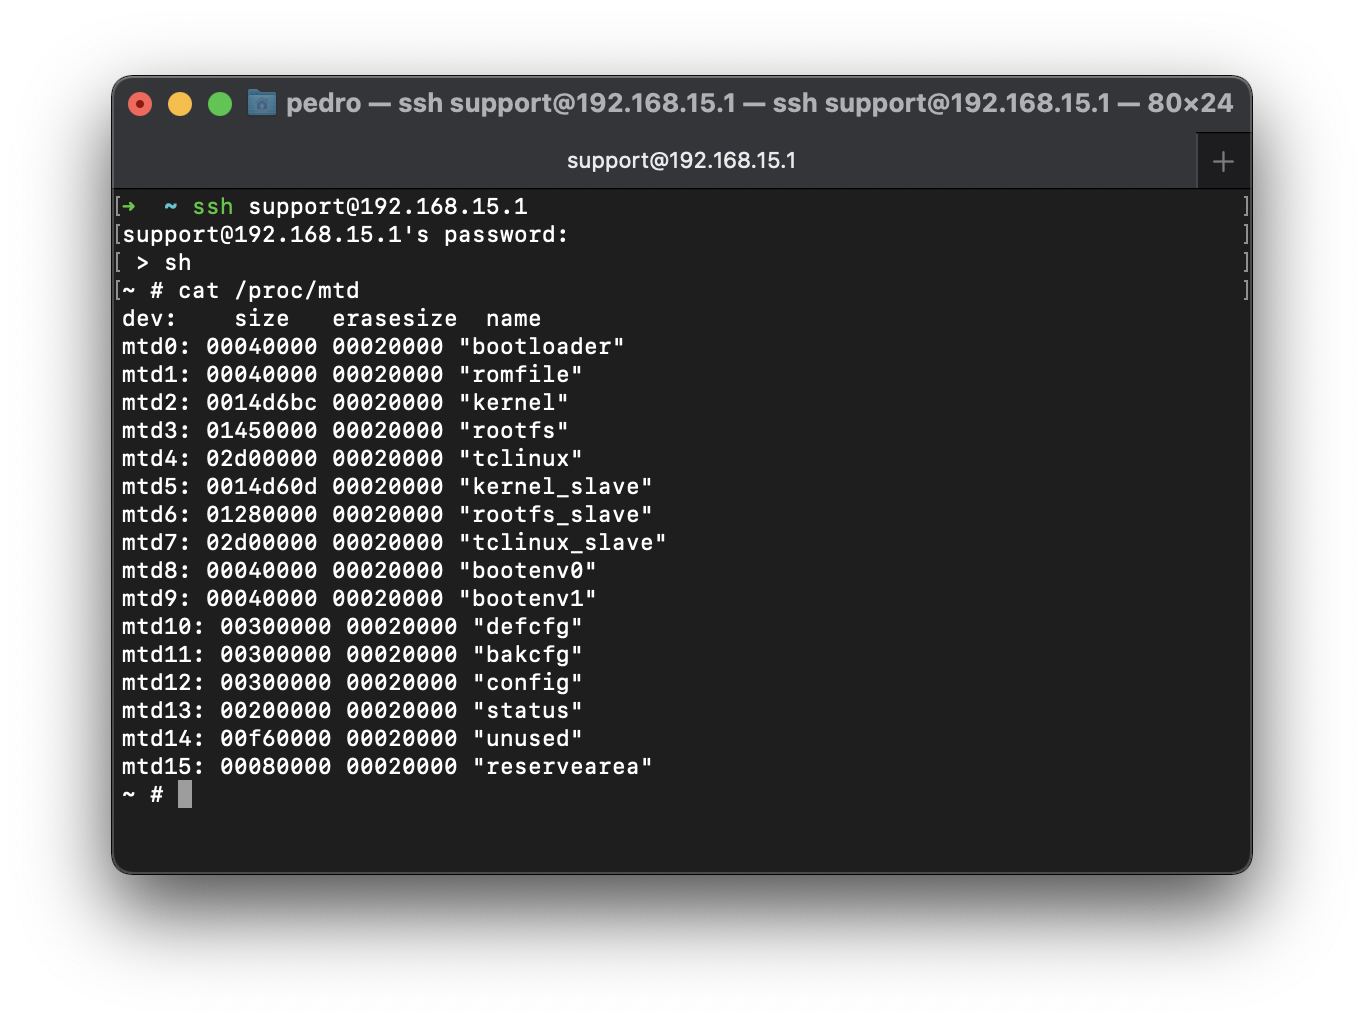
\includegraphics[width=\linewidth]{contents/cpes-and-research-data/eprom-extraction/cpe5-proc-mtd.png}
    \caption{File /proc/mtd of \gls{cpe} 5}
    \label{figure:cpe5_proc_mtd}
\end{figure}

Although it is possible to read the \gls{eprom} of \gls{cpe} 6 using the \gls{tftp} technique, the device’s shell sets a small time limit to processes executed from it, making it impossible to complete the transfer before the limit exceeds. To work around this problem, an \gls{eprom} programmer was directly attached to the \gls{cpe}’s \gls{eprom}, allowing a computer to dump its contents via the programmer.

On \glspl{cpe} 0 and 1, there is a command that shows the memory addresses where the \gls{eprom} is mapped and there is another command is capable of reading the content of an arbitrary memory address. Combining both commands, it is possible to extract the full \gls{eprom} content from a machine capable of accessing the \glspl{cpe} via Telnet. The scripts used are attached on Appendix \ref{appendix:cpe_eprom_ext}.

For \glspl{cpe} 2 and 3, the same technique of using an \gls{eprom} programmer had to be used. No command capable of dumping the \gls{eprom} via software was found.

\FloatBarrier
